\documentclass[letterpaper, 10pt]{article}

% Set margins 1 inch margins
\usepackage[a4paper,top=1in,bottom=1in,left=1in,right=1in]{geometry}
\usepackage{tikz}
\usepackage{pgfplots}
\usepackage{tabularx}

% Set double-spacing
\usepackage{setspace}
\doublespacing

% Use fancyhdr package
\usepackage{fancyhdr}
\setlength{\headheight}{1em}
\pagestyle{fancyplain}
\lhead{Dan Shea}
\chead{BIOL6308 - Bioinformatics Notes}
\rhead{\today}

% Don't indent paragraphs, place 1em between paragraphs
\setlength{\parindent}{0cm} % Default is 15pt.
\setlength{\parskip}{1em}

% Begin the document
\begin{document}
DNA can be displayed as sequences defined by 4 nucleotides:\\
\begin{tabular}{|l|l|}
\hline
\textbf{Purines} & \textbf{Pyrimidines}\\
\hline
\color{red}A\color{black}---Adenosine & \color{blue}T\color{black}---Thymine\\
\hline
\color{orange}C\color{black}---Cytosine & \color{purple}G\color{black}---Guanine\\
\hline
\end{tabular}\\\\
An \textbf{exon} is a stretch of DNA retained in mature mRNA on hat ribsome that translates into protein.\\
An \textbf{intron} is defined as intervening region between two exons.\\\\
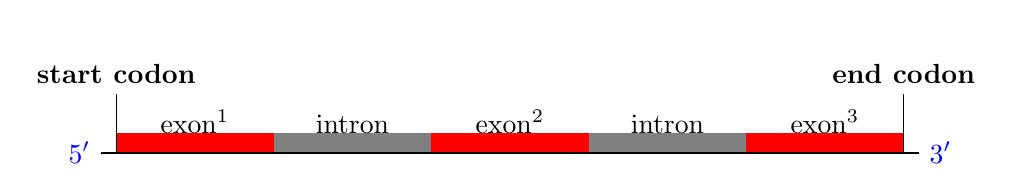
\begin{tikzpicture}
\fill [color=red] (0.2,0) rectangle (2.2,.25) node[midway, above, black]{exon$^1$};
\fill [color=gray] (2.2,0) rectangle (4.2,.25) node[midway, above, black]{intron};
\fill [color=red] (4.2,0) rectangle (6.2,.25) node[midway, above, black]{exon$^2$};
\fill [color=gray] (6.2,0) rectangle (8.2,.25) node[midway, above, black]{intron};
\fill [color=red] (8.2,0) rectangle (10.2,.25) node[midway, above, black]{exon$^3$};
\draw (0.2,0) -- (0.2,0.75) node[above, black]{\textbf{start codon}};
\draw (10.2,0) -- (10.2,0.75) node[above, black]{\textbf{end codon}};
\draw [thick, black] (0,0) node[left,blue]{$5'$} -- (10.4,0)node[right,blue]{$3'$};
\end{tikzpicture}\\
A \textbf{codon} consists of a sequence of three nucleotides.\\

\begin{tikzpicture}
\draw [red] (0,0) -- (0,-.25) -- (1,-.25) node[midway, above, black]{ATG} -- (1,0);
\end{tikzpicture}\\
\textbf{Sensitivity} $S_n$ is the measurement of \% of False Negatives (FN)\\
$S_n=\frac{TP}{TP+FN}$\\
\textbf{Specificity} $S_p$ is the measurement of \% of False Positives (FP)\\
$S_p=\frac{TN}{TN+FP}$\\
\textbf{Precision} is the measurement of \% of positives\\
A \textbf{ROC} plot (Receiver Operating Condition) is a plot of a classifier's behaviour over the range of the classifier's variable parameters.\\\\
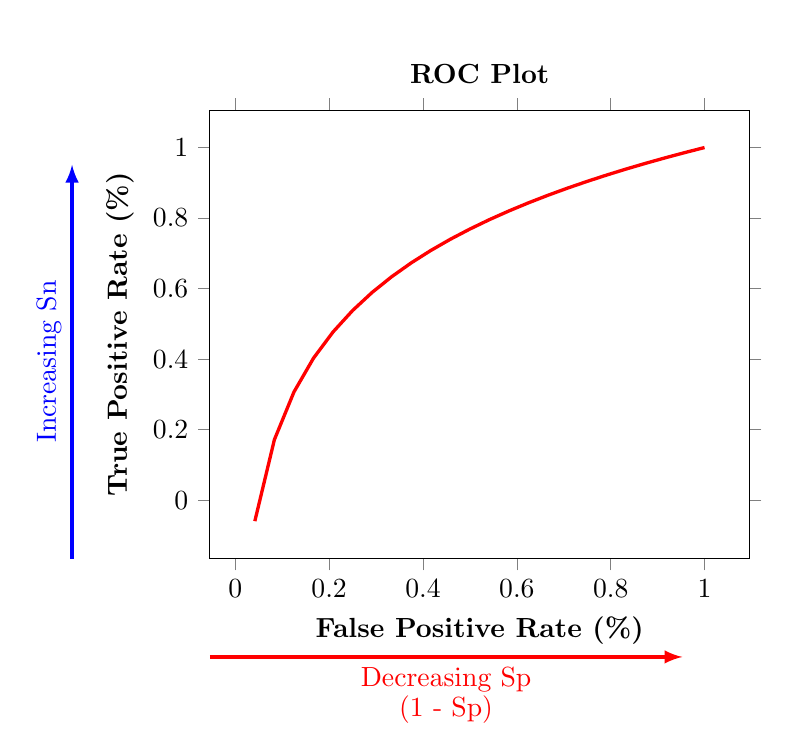
\begin{tikzpicture}
	\begin{axis}[
		title=\textbf{ROC Plot},
		tick align=outside,
		xlabel=\textbf{False Positive Rate (\%)},
		ylabel=\textbf{True Positive Rate (\%)},]
		\addplot[domain=0:1, color=red, very thick] {(ln(x)+3)*(1/3)};
	\end{axis}
	\draw [very thick, blue, >=latex, ->] (-1.75,0) -- (-1.75,5) node[sloped,midway,above]{Increasing Sn};
	\draw [very thick, red, >=latex, ->] (0,-1.25) -- (6,-1.25) node[midway,below]{Decreasing Sp}
															   node[midway,below,yshift=-10]{(1 - Sp)};
\end{tikzpicture}
\end{document}